%

\section{Introduction}

In this chapter we illustrate that stochastic planning can be viewed
as a specific form of probabilistic inference and show that recent symbolic
dynamic programming (SDP) algorithms for the planning problem can be
seen to perform  ``generalized lifted
inference'', thus making a strong connection to other chapters in this
book.  As we discuss below, although the SDP formulation is more
expressive in principle, work on SDP to date has largely focused on
algorithmic aspects of reasoning in open domain models with rich
quantified logical structure whereas lifted inference has largely
focused on aspects of efficient arithmetic computations
over finite domain (quantifier free) template-based models.
The contributions in these areas are therefore largely along different dimensions.
%
%
%
%
%
%
%
%
%
%
%
%
%
%
%
%
%
%
%
%
%
However, the intrinsic relationships between these problems
suggest a strong opportunity for cross-fertilization where the
true scope of generalized lifted inference can be achieved.  This
chapter intends to highlight these relationships and 
lay out a paradigm for generalized lifted inference that subsumes both
fields and offers interesting opportunities for future research.

%
%

To make the discussion concrete, let us introduce a running example for stochastic
planning and the kind of generalized solutions that can be achieved.
For illustrative purposes, we borrow a planning domain from Boutilier
et.\ al.~\cite{BoutilierRePr01} that we refer to as \textsc{BoxWorld}.
In this domain, outlined in Figure~\ref{fig:boxworld}, there are
several cities such as $\london$, $\paris$ etc., trucks $\truck_1$,
$\truck_2$ etc., and boxes $\tbox_1$, $\tbox_2$ etc. The agent can load
a box onto a truck or unload it and can drive a truck from one city to
another.  When any box 
%
has been delivered to a
specific city, $\paris$, the agent receives a positive
reward.  The agent's planning task is to find a policy for action
selection that maximizes this reward over some planning horizon.

%
%
%
%
%
%

%
%
\begin{figure}[t!]

\caption{A formal desciption of the \textsc{BoxWorld} adapted
  from~\cite{BoutilierRePr01}. We use a simple STRIPS-like~\cite{strips}
  add and delete list representation of actions and, as a simple
  probabilistic extension in the spirit of PSTRIPS~\cite{pso}, we
  assign probabilities that an action successfully executes
  conditioned on various state properties.\label{fig:boxworld}}
\vspace{2mm}
\begin{center}
\fbox{\begin{minipage}{\columnwidth}
{
%
\centering \small 
\begin{itemize} 
\item {\it Domain Object Types (i.e., sorts)}: $\TBox$, $\Truck$, $\City = \{ \paris, \ldots \}$
\item {\it Relations (with parameter sorts)}: \\BoxIn: $\BIn(\TBox,\City)$, TruckIn: $\TIn(\Truck,\City)$, BoxOn: $\On(\TBox,\Truck)$
\item {\it Reward}: if $\exists B, \BIn(B,\paris)$ then 10 else 0
\item {\it Actions (with parameter sorts)}:
  \begin{itemize} \denselist
  \item $\load(\TBox:B,\Truck:T,\City:C)$: %
    %
    %
    \begin{itemize} \denselist
    \item Success Probability: if $(\BIn(B,C) \wedge \TIn(T,C))$ then .9 else 0
    \item Add Effects on Success: $\{ \On(B,T) \}$
    \item Delete Effects on Success: $\{ \BIn(B,C) \}$
    \end{itemize}
  \item $\unload(\TBox:B,\Truck:T,\City:C)$: %
    \begin{itemize} \denselist
    \item Success Probability: if $(\On(B,T) \wedge \TIn(T,C))$ then .9 else 0
    \item Add Effects on Success: $\{ \BIn(B,C) \}$
    \item Delete Effects on Success: $\{ \On(B,T) \}$
    \end{itemize}
  \item $\drive(\Truck:T,\City:C_1,\City:C_2)$:
    \begin{itemize} \denselist
    \item Success Probability: if $(\TIn(T,C_1))$ then 1 else 0
    \item Add Effects on Success: $\{ \TIn(T,C_2) \}$
    \item Delete Effects on Success: $\{ \TIn(T,C_1) \}$
    \end{itemize}
  \item $noop$
    \begin{itemize} \denselist
    \item Success Probability: 1
    \item Add Effects on Success: $\emptyset$
    \item Delete Effects on Success: $\emptyset$
    \end{itemize}
  \end{itemize}
\end{itemize}}
\end{minipage}}
\end{center}
\end{figure}
%

Our objective in lifted stochastic planning is to obtain an
abstract policy, for example, like the one shown in Figure~\ref{fig:vfun_and_policy}.
In order to get some box to $\paris$, the agent should drive a truck
to the city where the box is located, load the box on the truck, drive
the truck to $\paris$, and finally unload the box in $\paris$.  This
is essentially encoded in the symbolic value function shown in
Fig.~\ref{fig:vfun_and_policy}, which was computed by discounting rewards
$t$ time steps into the future by $0.9^t$.

Similar to this example,
for some problems we can obtain a solution which is
described abstractly and is independent of the specific problem
instance or even its size --- for our example problem the description of
the solution does not depend on the number of cities, trucks or boxes, or
on  knowledge of the particular location of any specific truck.
Accordingly, one might hope that computing such a solution can be done without knowledge of these quantities and in time complexity independent of them.
This is the computational advantage of symbolic stochastic planning
which we associate with lifted inference in this chapter. 

The next two subsections expand on the connection between planning and inference, identify opportunities for lifted inference, and use these observations to define a new setup which we call {\em generalized lifted inference} which abstracts some of the work in both areas and provides new challenges for future work. 


%
%
%
%
%
%
%
%
%
%
%
%
%

%
%
%
%
%
%

%
%
%
%
%

%
%
\begin{figure}[t!]
\caption{A decision-list representation of the optimal policy and 
  expected discounted reward for the \textsc{BoxWorld} problem.
  The optimal action parameters in the \emph{then} conditions correspond to the existential
  bindings that made the \emph{if} conditions true.
  \label{fig:vfun_and_policy}
}
\vspace{2mm}
\begin{center}
\fbox{\begin{minipage}{\columnwidth}
{
%
 \small
if $(\exists B, \BIn(B,\paris))$ then do $\noop$ (value = 100.00)\\
else if $(\exists B,T, \TIn(T,\paris) \wedge \On(B,T))$ then do $\unload(B,T,\paris)$ (value = 89.0)\\
else if $(\exists B,C,T, \On(B,T) \wedge \TIn(T,C))$ then do $\drive(T,C,\paris)$ (value = 80.0)\\
else if $(\exists B,C,T, \BIn(B,C) \wedge \TIn(T,C))$  then do $\load(B,T,C)$ (value = 72.0)\\
else if $(\exists B,C_1,T,C_2, \BIn(B,C_1) \wedge \TIn(T,C_2))$ then do $\drive(T,C_2,C_1)$ (value = 64.7)\\
else do $\noop$ (value = 0.0)
}
\end{minipage}}
\end{center}\end{figure}
%

\subsection{Stochastic Planning and Inference}

%
%
%
%
%
%

Planning is the task of choosing what actions to take to achieve some
goals or maximize long-term reward.  When the dynamics of the world are 
deterministic, that is, each action has exactly one known outcome,
then the problem can be solved through logical inference. That is,
inference rules can be used to deduce the outcome of individual actions given the
current state, and by combining inference steps one can prove that the
goal is achieved. In this manner a proof of goal achievement embeds a
plan. This correspondence was at the heart of McCarthy's
seminal paper \cite{McCarthy58} that introduced the topic of AI and viewed
planning as symbolic logical inference.  Since this formulation uses
first-order logic, or the closely related situation calculus, lifted
logical inference can be used to solve deterministic planning
problems.

When the dynamics of the world are non-deterministic, this
relationship is more complex.  In particular, in this chapter we focus
on the stochastic planning problem where an action can have multiple
possible known outcomes that occur with known state-dependent
probabilities.  Inference in this case must reason about probabilities
over an exponential number of state trajectories for some
planning horizon.
%
%
%
While lifted inference and planning may seem to be entirely different
problems, analogies have been made between the two fields in several
forms~\cite{Attias03,ToussaintSt06,domshlak2006,LangTo09,FurmstonB10,LiuI12,ChengLCI13,LeeMaDe14,LeeMaDe16,issakkimuthu2015hop,MeentPTW16}.
To make the connections concrete, consider a finite domain and the finite
horizon goal-oriented version of the \textsc{BoxWorld} planning
problem of Figure~\ref{fig:boxworld}, e.g., two boxes, three trucks,
and four cities and a planning horizon of 10 steps where the goal is
to get some box in $\paris$.  In this case, 
the value of a state, $V(S)$, corresponds to the probability of
achieving the goal, and
goal achievement can be
modeled as a specific form of inference in a Bayesian network or
influence diagram.  

We start by considering the {\em conformant planning problem} where 
the intended solution is an explicit sequence of actions.
%
In this case, the sequence of actions is determined in advance and 
action choice at the $i$th step does not depend on the actual state at the $i$th step.
For this formulation,
one can build a Dynamic Bayesian Network (DBN) model where
each time slice represents the state at that time and action nodes
affect the state at the next time step, as in
Figure~\ref{fig:PasI}(a).  The edges in this diagram capture
$p(S'|S,A)$, where $S$ is the current state, $A$ is the current action
and $S'$ is the next state, and each of $S,S',A$ is represented by
multiple nodes to show that they are given by a collection of
predicates and their values.  Note that, since the world dynamics are
known, the conditional probabilities for all nodes in the graph
are known. 
As a result, 
the goal-based planning problem where a goal $G$ must hold at the last step,
can be modeled using standard
inference. The value of conformant planning is given by marginal MAP (where
we seek a MAP value for some variables but take expectation over the remaining variables)
\cite{domshlak2006,LeeMaDe14,LeeMaDe16}:
\begin{eqnarray*}
%
V_{\mbox{\footnotesize{conformant}}}(S_0) 
& = & \max_{A_0}, \ldots, \max_{A_{N-1}} 
Pr( G | S_0, A_0, \ldots, A_{N-1})  \\
& = & \max_{A_0}, \ldots, \max_{A_{N-1}} 
\sum_{S_1,S_2,\ldots,S_{N}} 
Pr( G,S_1,\ldots,S_N | S_0, A_0, \ldots, A_{N-1}). 
\end{eqnarray*}
The optimal conformant plan is extracted using
argmax instead of max in the equation.

The standard MDP formulation with a reward per time time step which is accumulated can be handled similarly, by normalizing the cumulative reward and adding a binary node $G$ whose probability of being true is a function of the normalized cumulative reward. Several alternative formulations of planning as inference have been proposed by defining an auxiliary distribution over finite trajectories which captures utility weighted probability distribution over the trajectories \cite{ToussaintSt06,FurmstonB10,LiuI12,ChengLCI13,MeentPTW16}. While the details vary, the common theme among these approaches is that the planning objective is equivalent to calculating the partition function (or ``probability of evidence") in the resulting distribution. 
This achieves the same effect as adding a node $G$ that depends on the cumulative reward.
To simplify the discussion, we continue the presentation with the simple goal based formulation. 


The same problem can be viewed from a Bayesian perspective, treating actions as random variables with an uninformative prior. In this case we can use
\[
Pr(G | S_0, A_0, \ldots, A_{N-1}) = 
\frac
{Pr(A_0, \ldots, A_{N-1}| G, S_0 ) Pr(G | S_0)}{Pr(A_0, \ldots, A_{N-1}|  S_0)}.
\]
to observe that  \cite{Attias03,ToussaintSt06,LangTo09}
\[
\argmax_{A_0}, \ldots, \max_{A_{N-1}}  Pr(G | S_0, A_0, \ldots, A_{N-1}) = \argmax_{A_0}, \ldots, \max_{A_{N-1}}  Pr(A_0, \ldots, A_{N-1}| G, S_0 )
\]
and therefore one can alternatively maximize the probability conditioned on $G$.


\begin{figure*}
\begin{center}
%
\fbox{
\begin{minipage}{2.1in}
\begin{center}
{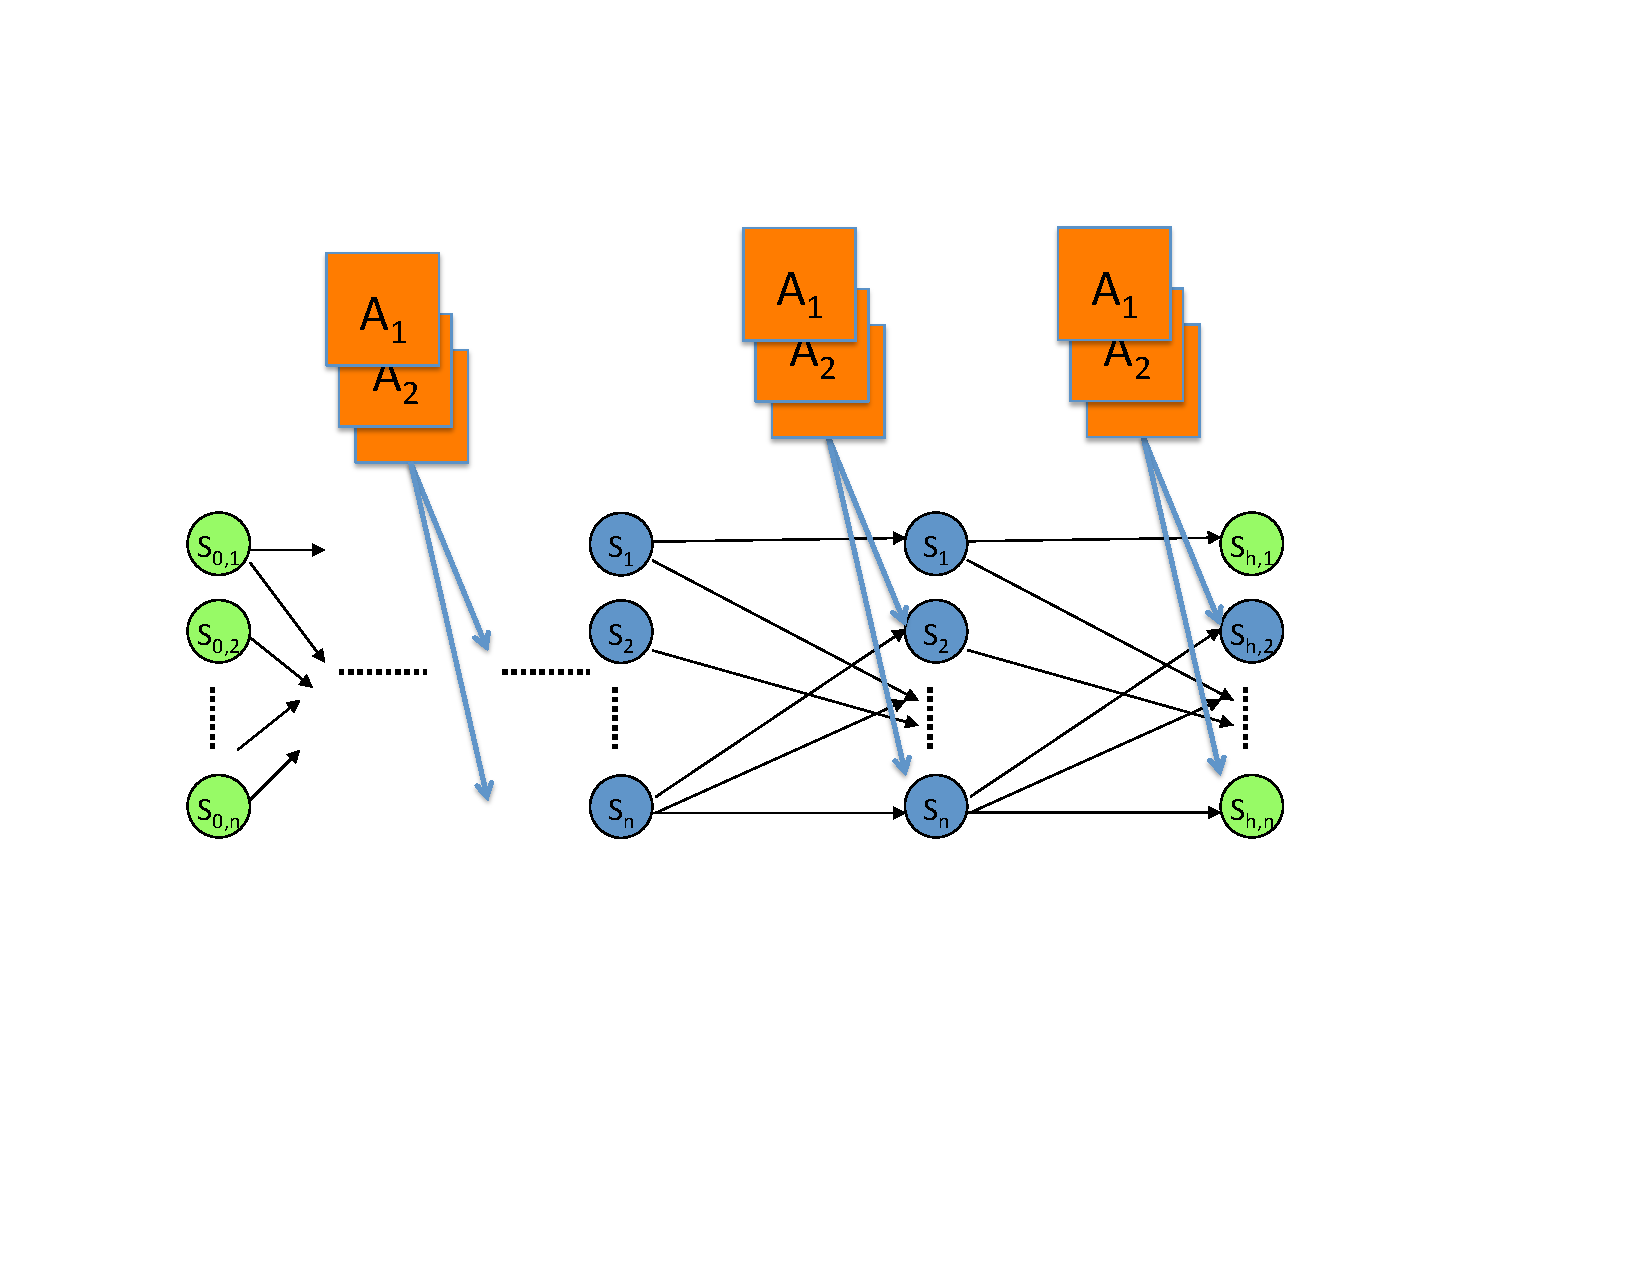
\includegraphics[height=1.1in,angle=0]{\ChapterPath/dbn-conformant}}

(a)
\end{center}
\end{minipage}
}
\fbox{
\begin{minipage}{2.1in}
\begin{center}
{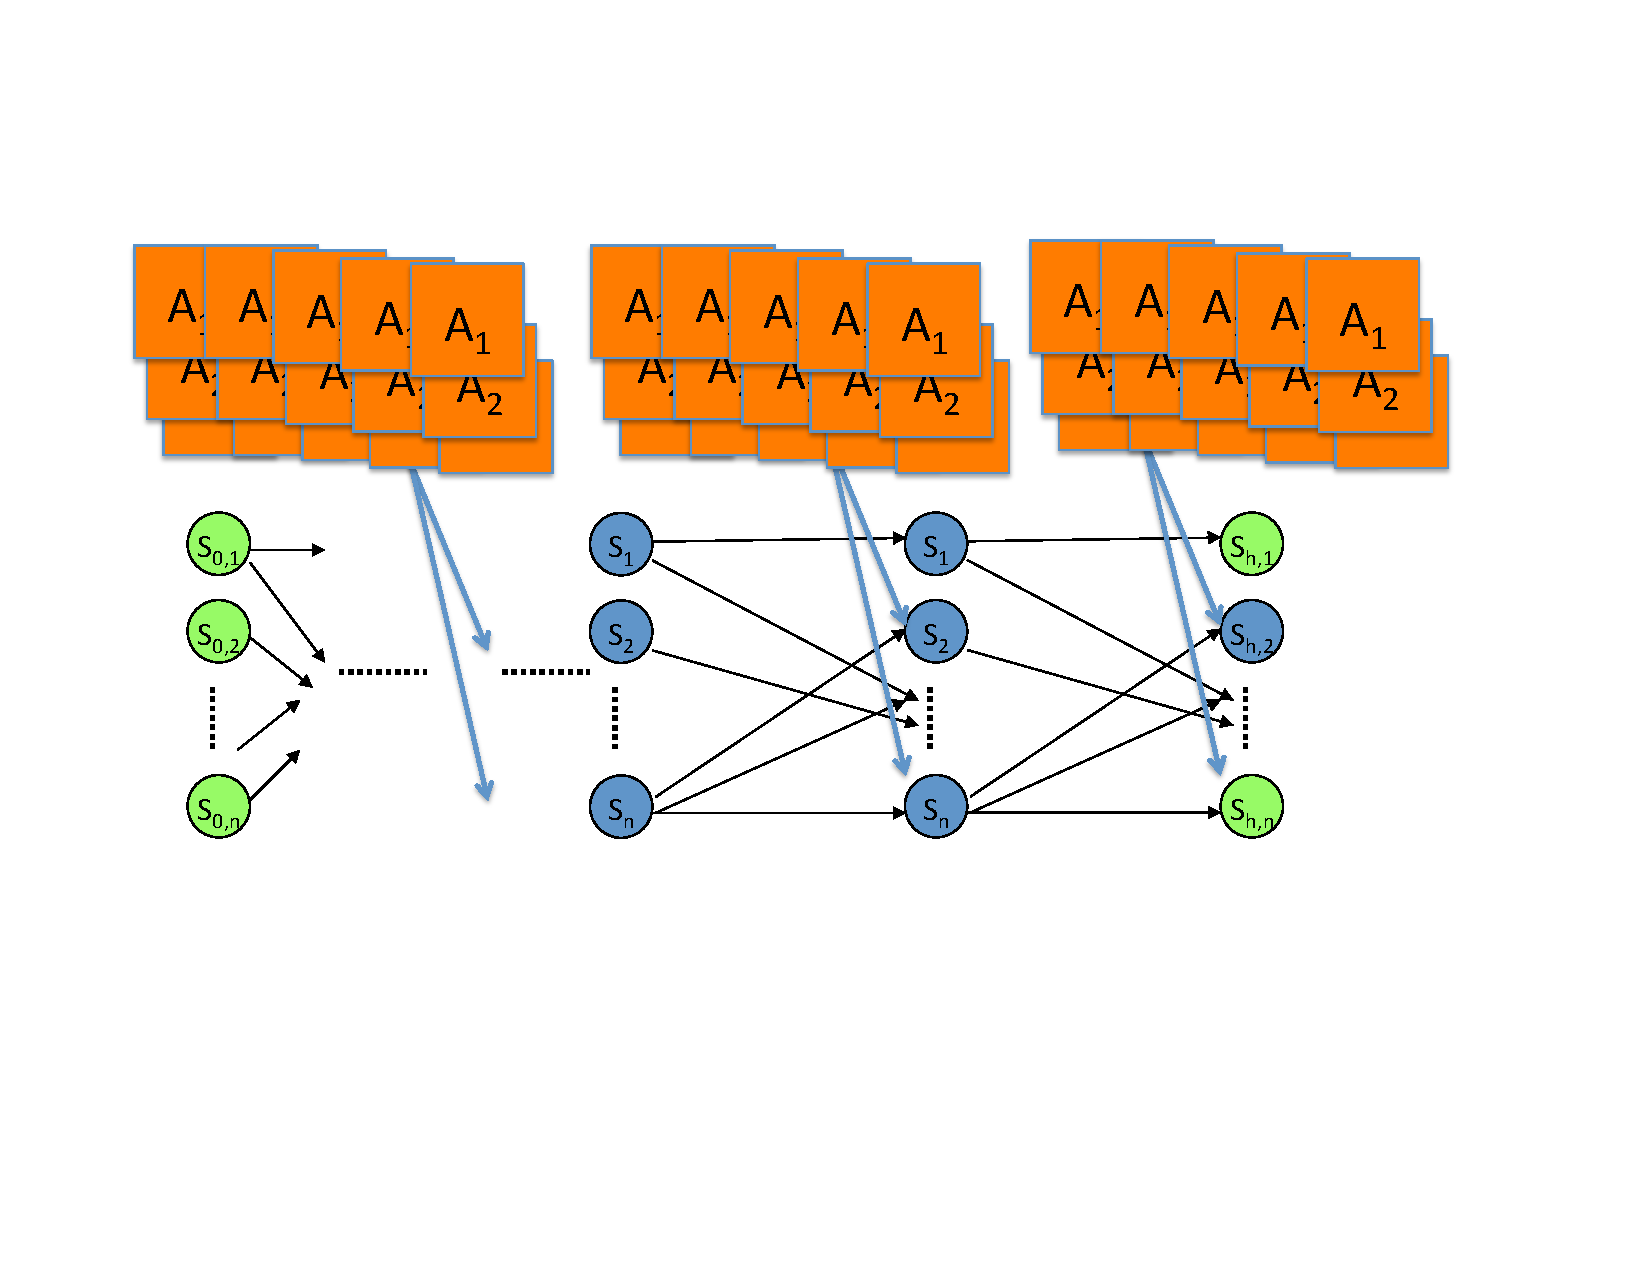
\includegraphics[height=1.1in,angle=0]{\ChapterPath/dbn-policy}}

(b)
\end{center}
\end{minipage}
}
\end{center}
\caption{Planning as inference: conditioning on start and goal state.
(a) Conformant planning -- actions selected per time step without knowledge of the state.
(b) An exponential size policy at each time step determines action selection. The transition depends on the current state and policy's actions for that state.
%
%
  %
  %
  %
}
\label{fig:PasI}
\end{figure*}

However, linear plans, as the ones produced by the conformant setting, are not optimal for probabilistic planning. In
particular, if we are to optimize goal achievement then we must allow
the actions to depend on the state they are taken in. That is, the
action in the second step is taken with knowledge of the probabilistic
outcome of the first action, which is not known in advance. 
We can achieve this by duplicating action nodes, with a copy for each possible value of the state variables, as illustrated in 
Figure~\ref{fig:PasI}(b). This represents a separate policy associated with each horizon depth which is required because finite horizon problems have non-stationary optimal policies.
In this case, state transitions depend on the identity of the current state and the action variables associated with that state. 
%
%
%
%
%
%
%
%
%
%
%
%
%
%
%
%
%
The corresponding inference problem can
be written as follows:
\begin{equation}
\label{eq:VoptV1}
V(S_0) = \max_{A_0(S_0)}, \ldots, \max_{A_{N-1}(S_N-1)} Pr(G | S_0, A_0(S_0), \ldots, A_{N-1} (S_N-1 ) ). 
\end{equation}
However, the number of random variables in this formulation is
prohibitively large since we need the number of original action variables to be multiplied by the size of the state space. 

Alternatively, the same desideratum, optimizing
actions with knowledge of the previous state, can be achieved without
duplicating variables in the equivalent formulation
\begin{align}
V(S_0) &  = 
\max_{A_0}
\sum_{S_1}
Pr(S_{1}|S_{0},A_{0})
\max_{A_1}
\sum_{S_2}
Pr(S_{2}|S_{1},A_{1})
\ldots
\nonumber
\\
& \ \ \ \ 
\max_{A_{N-2}}
\sum_{S_{N-1}}
Pr(S_{N-1}|S_{N-2},A_{N-2})
\max_{A_{N-1}}
\sum_{S_N}
Pr(S_N|S_{N-1},A_{N-1})
Pr(G|S_n). 
\label{eq:VoptV2}
\end{align}
In fact, this formulation is exactly the same as the finite horizon
application of the value iteration (VI) algorithm for (goal-based) Markov Decision
Processes (MDP) which is the standard formulation for sequential decision
making in stochastic environments.  The standard formulation abstracts
this by setting 
\begin{align}
V_0(S) & = Pr(G|S) 
\nonumber
\\
V_{k+1}(S) & =  
\max_{A}
\underbrace{\sum_{S'} Pr(S'|S,A) V_k(S')}_{Q(S,A)}.
\label{eq:VI} 
\end{align}
The optimal policy (at $S_0$) can be obtained as before by recording
the argmax values.  In terms of probabilistic inference, the problem
is no longer a marginal MAP problem because summation and maximization steps are
constrained in their interleaved order. But it can be seen as a natural extension of such inference questions with several alternating blocks of expectation and maximization.
We are not aware of an explicit study of such problems outside the planning context.


\subsection{Stochastic Planning and Generalized Lifted Inference}

Given that planning can be seen as an inference problem, one can try
to apply ideas of lifted inference to planning.  Taking the motivating
example from Figure~\ref{fig:boxworld}, let us specialize the reward
to a ground atomic goal $G$ equivalent to $\BIn(b^*,\paris)$ for
constants $b^*$ and $\paris$.  Then we can query
$\max_A Pr(\BIn(b^*,\paris)|s_0,A)$ to compute $V(S_0=s_0)$ where $s_0$ is
the concrete value of the current state.  

Given that
Figure~\ref{fig:boxworld} implies a complex relational specification
of the transition probabilities, lifted inference techniques are
especially well-placed to attempt to exploit the structure of this
query to perform inference in aggregate and thus avoid redundant
computations.
%
However, we emphasize that, even if lifted inference is used, this is a standard query in the graphical model where evidence constrains the value of some nodes, and the solution is a single number representing the corresponding probability (together with a MAP assignment to variables). 


%
%
%
%
%
%
%

%
%
However, Eq~\ref{eq:VI} suggests an explicit additional structure for
the planning problem. In particular, the intermediate expressions $V_k(S)$
include the values (the probability of reaching the goal in $k$ steps)
for all possible concrete values of $S$. Similarly, the final result
$V_N(S)$ includes the values for all possible start states. In addition, as in our running example we can consider more abstract rewards.
This suggests a
first generalization of the standard setup in lifted
inference. Instead of asking about a ground goal $Pr(\BIn(b^*,\paris))$ and expecting a single number as a response, we can abstract the setup in two ways: first, we can ask about
more general conditions such as $\exists B, Pr(\BIn(B,\paris))$ and second we can expect to get a structured result that specifies the
corresponding probability for every concrete state in the world.
%
%
%
If we had two box instances $b_1,b_2$ and $m$ truck instances $t_1,\ldots,t_m$, the answer for $V_1(S)$, i.e., the value for the goal based formulation with horizon one, might take the form:
\begin{center}
\vspace{-4mm}
%
%
%
%
%
%
%
%
%
%
%
\fbox{\begin{minipage}{\columnwidth}
{
%
if $(\BIn(b_1,\paris)\vee \BIn(b_2,\paris))$\\
$\mbox{\;}$ \hspace{10mm} then 
%
$V_1(S)=10$\\
else if $((\TIn(t_1,\paris) \!\wedge\! \On(b_1,t_1)) 
\!\vee\! 
\ldots \!\vee\! (\TIn(t_m,\paris) \!\wedge\! \On(b_2,t_m)))$\\
$\mbox{\;}$ \hspace{10mm} then 
%
$V_1(S)=9$\\
else 
$V_1(S)=0$.
%
}
\end{minipage}}
\end{center}
%
%
%
The significance of this is that the question can have a more general form and that the answer solves many problems simultaneously, providing the response as a case analysis depending on some properties of the state. 
We refer to this reasoning as {\em inference with
generalized queries and answers}.  In this context, the goal of lifted inference will
be to calculate a structured form of the reply directly. 

%
A second extension arises from the setup of generalized
queries. The standard form for lifted inference is to completely
specify the domain in advance. This means providing the number of
objects and their properties, and that the response to the query is calculated
only for this specific domain instantiation.
%
%
%
%
%
%
However, inspecting the solution in the previous paragraph it is obvious that we can at least hope to do better. The same solution can be described more compactly as 
\begin{center}
\vspace{-4mm}
\fbox{\begin{minipage}{\columnwidth}
{
if $(\exists B, \BIn(B,\paris))$\\
$\mbox{\;}$ \hspace{10mm} then 
$V_1(S)=10$\\
else if $(\exists B,\exists T, (\TIn(T,\paris) \!\wedge\! \On(B,T))$ \\
$\mbox{\;}$ \hspace{10mm} then 
$V_1(S)=9$\\
else 
$V_1(S)=0$.
}
\end{minipage}}
\end{center}
Arriving at such a solution requires us to 
allow open domain reasoning over all potential objects (rather than
grounding them, which is impossible in open domains), and to extend 
ideas of lifted inference to exploit quantifiers and their structure. 
Following through with this idea, we can 
%
%
%
%
arrive at a \emph{domain-size independent value function and policy}
as the one shown in Figure~\ref{fig:vfun_and_policy}.  
In this context, the goal of lifted inference will
be to calculate an abstracted form of the reply directly. 
We call this problem {\em inference with generalized models}.
As we describe in this chapter, SDP algorithms are able to perform this type of inference.

The previous example had enough structure and a special query that allowed the solution to be specified without any knowledge of the concrete problem instance. This property is not always possible.  
%
For example, consider a setting 
where we get one unit of reward for every box in $\paris$: 
$\sum_{B:\TBox} \mbox{[if $(\BIn(B,\paris))$ then 1 else 0]}$.
In addition, consider the case where, after the agent takes their action, any box which is not on a truck disappears with probability $0.2$.
In this case, we can still potentially calculate an abstract solution, but it requires access to more complex properties of the state, and in some cases the domain size (number of objects) in the state. For our example this gives:
\begin{center}
\vspace{-4mm}
\fbox{\begin{minipage}{\columnwidth}
{
Let $n=(\#_B, \BIn(B,\paris))$\\
if $(\exists B,\exists T, (\TIn(T,\paris) \!\wedge\! \On(B,T))$ \\
$\mbox{\;}$ \hspace{10mm} then 
$V_1(S)=n*8+ 7.2$\\
else 
$V_1(S)=n*8$.
}
\end{minipage}}
\end{center}
Here we have introduced a new notation for count expressions where, for example, $(\#_B, \BIn(B,\paris))$ counts the number of boxes in Paris in the current state. 
To see this result note that any existing box in Paris disappears 20\% of the time and that
a box on a truck is successfully unloaded 90\% of the time but remains and does not disappear only in 80\% of possible futures leading to the value 7.2.
This is reminiscent of the type of expressions that arise in existing lifted inference problems and solutions. 
Typical solutions to such problems
%
%
%
%
involve parameterized expressions over the domain (e.g., counting, summation, etc.),
and critically do not always require closed-domain reasoning (e.g., \textit{a priori}
knowledge of the number of boxes).  They are therefore suitable for inference with generalized models.
Some work on SDP has approached lifted inference for problems with this level of complexity, including exogenous activities (the disappearing boxes) and additive rewards.
But, as we describe in more detail, the solutions for these cases are much less well understood and developed. 


%
%
%
%
%
%

To recap, our example illustrates that stochastic planning potentially enables abstract solutions that 
might be amenable to lifted computations. 
SDP solutions for planning problems have
focused on the computational advantages arising from these
expressive generalizations. At the same time, the focus in SDP algorithms has largely been on
problems where the solution is completely independent of domain size and does not require numerical properties of the state. 
These algorithms have thus skirted some of
the computational issues that are typically tackled in lifted inference. It is the
combination of these aspects, as illustrated in the last example, which we call {\bf generalized lifted
inference}. As the discussion suggests, generalized lifted inference is still very much an open problem. In addition to providing a survey of existing SDP algorithms, the goal of this chapter is to highlight the opportunities and challenges in this exciting area of research.

%
%

\commentout{
Given that planning can be seen as an inference problem, one can try
to apply ideas of lifted inference to this problem. Let us consider
the analogy, by relating to a problem from Chapter 1. \mycomment{refer
  to a concrete simple lifted inference problem} In this case, given a
compact relational specification of the problem and some evidence one
seeks the marginal probability of some atom $p(rich(Joe))$. The answer
to this query is a single number providing this probability.
similarly, in Eq~(\ref{eq:VoptV2}) we seek a single number specifying
$V(S_0=s_0)$ where $s_0$ is the concrete value of the current
state. In such application, we seek to speed up the computation by
taking advantage of structure in the model $p(s'|s,a)$ to avoid
recompilation and aggregate values where possible.

However, Eq~\ref{eq:VI} suggests an explicit additional structure for
the planning problem. In particular, the intermediate values $V_k(S)$
include the values (the probability of reaching the goal in $k$ steps)
for all possible concrete values of $S$. Similarly, the final result
$V_N(S)$ includes the values for all start states. This suggests a
first generalization of the standard setup in lifted
inference. Instead of asking about $p(rich(Joe))$ we can ask about
$p(rich(X))$ and get a structured result the specifies the
corresponding probability for every concrete object $X$ in the
domain. The answer might take the form: [if $parent(X,Y) \wedge
  rich(Y)$ then $p(rich(X))=0.9$ else \ldots else
  $p(rich(X))=0.01$]. In the context of planning problems the variable
$X$ ranges over states which is typically much larger than the number
of individuals as in this example.  We refer to this as {\bf inference
  with generalized queries and answers}. Here lifted inference will
attempt to calculate a structured form of the reply to all the
queries.

A second generalization arises from the setup of generalized
queries. The standard form for lifted inference is to completely
specify the domain in advance. This means providing the number of
objects and their properties and that $p(rich(Joe))$ is calculated
only for this specification. \mycomment{for this point it would be
  good to have two variants of the basic problem p(rich(Joe)) --- one
  where the answer does not depend on the number of objects, and one
  where it does depend but the dependence is parametric so we can give
  a symbolic answer. Perhaps a horizon 2 planning goal will do the
  trick.}. However, if we consider problem 1 in our example we see
that the answer does not depend on the domain size. Problem 2
similarly illustrates that we can provide a symbolic answer.  A
related aspect arises in planning model where the reward is often an
additive function over the domain but it does not require an explicit
specific of domain size. For example, an inventory control problem
might award a negative reward for each empty shop in the current
state: this can be written as $\sum_{s:\mbox{Shop}} empty(s)$. Here
the total reward and value functions are a function of the concrete
number of shops but the model specification and the solution may be
specified using parameterized expressions over the domain.  In both
cases, we can relax the requirements on the input specification (to
omit size) or provide it in parameterized form yielding the problem we
call {\bf inference with generalized models}.
}













